\chapter{Transformação de funções}

Podemos fazer várias mudanças nas funções de forma que seus com gráficos mudem de maneira previsível. É possível movê-los para cima e para baixo ou para os lados. Também podemos fazer espelhamentos no eixo horizontal e vertical. Por último, é possível esticar ou encolher os gráficos.

A seguir, vamos falar sobre as diferentes maneiras de alterar os gráficos das funções.

 \section{Translação vertical}

 Vejamos o seguinte exemplo:

 \begin{exem}
  Considere a função $f(x): \R \to \R$, dada por $f(x)= x^2$. Defina as seguintes funções $g,h: \R \to \R$ dadas por 
  \begin{align*}
        g(x) &= f(x) + 2= x^2 + 2,\\
        h(x) &= f(x) - 2= x^2 - 2.
  \end{align*}
  
    Observe na seguinte figura como estas transformações alteram o gráfico da função $f$:
    
    \begin{center}
  \begin{tikzpicture}[scale=0.7]
    \tkzInit[xmin=-4, xmax=4, ymin=-3,ymax=5]
        %\tkzDrawXY
        \tkzAxeXY[fill=black!5]
        %\tkzLabelX[text=blue,below = 3pt,]
        
        \tkzFct[thick,red]{x**2}
        \tkzText[above left, red](1.4,1){$f(x)$}

        \tkzFct[thick,blue]{x**2+2}
        \tkzText[above left, blue](1.4,3){$g(x)$}

        \tkzFct[thick,blue]{x**2-2}
        \tkzText[below right, blue](0.8,-1){$h(x)$}
        
        %\tkzFct[thick,red]{x**3}
        %\tkzFct[thick,red,domain=-1.5:1.5]{x**5}

        %\tkzDefPoint(1.5,0.25){A}
        %\tkzDefPointByFct[ref=A, with=a](-1)
        %\tkzDefPoint(0,2){A}
        %\tkzDefPoint(0.5,2.25){B}
        %\tkzPointShowCoord[xlabel=$\frac{3}{2}$]((1.5,0.25))
        %\tkzDrawPoint[fill=red, size=3](A)
        %\tkzDrawPoint[fill=red, size=3](B)
        
    \end{tikzpicture}
\end{center}

    Note a função $g$ carregou o gráfico da $f$ duas unidades ``para cima'' no eixo $y$, já a função $h$ carregou o gráfico da $f$ duas unidades ``para baixo'' no eixo $y$.

%  \begin{figure}[H]
%    \fbox{\subfigure[Gráficos das funções $f$ e $g$]{\includegraphics[width=7cm,height=6cm]{./cap_funcao/figs/translacaomais2}}}
%    \fbox{\subfigure[Gráficos das funções $f$ e $h$]{\includegraphics[width=7cm,height=6cm]{./cap_funcao/figs/translacaomenos2}}}
% \caption{Translação no eixo $y$}
%   \end{figure}
 \end{exem}

\begin{obs}
Suponha que $c>0$.
\begin{itemize}
    \item Para o obter o gráfico de $y=f(x)+c$, desloque o gráfico de $f(x)$ em $c$ unidades para cima;
    \item Para obter o gráfico de $y=f(x)-c$, desloque o gráfico de $f(x)$ em $c$ unidades para baixo.
\end{itemize}
\end{obs}


 %Dados $A, B \subset \R$ e uma função $f(x): A \to B$, definimos a função translação de $f$ no eixo $y$, pela função $g(x): A \to B$, dada por \destaque{g(x)= f(x) + c}, onde $c \in \R$ é uma constante.

 \section{Translação horizontal}

  Considere o seguinte exemplo:

 \begin{exem}
  Seja $f(x): \R \to \R$, dada por $f(x)= x^2$. Defina as seguintes funções $g,h: \R \to \R$ dadas por 
  \begin{align*}
        g(x) &= f(x+2)= (x+2)^2,\\
        h(x) &= f(x-2)= (x-2)^2.
  \end{align*}
  
    Observe na seguinte figura como estas transformações alteram o gráfico da função $f$:

    \begin{center}
  \begin{tikzpicture}[scale=0.7]
    \tkzInit[xmin=-4, xmax=4, ymin=-3,ymax=5]
        %\tkzDrawXY
        \tkzAxeXY[fill=black!5]
        %\tkzLabelX[text=blue,below = 3pt,]
        
        \tkzFct[thick,red]{x**2}
        \tkzText[above right, red](1.6,2){$f(x)$}

        \tkzFct[thick,blue]{(x+2)**2}
        \tkzText[above right, blue](-3,1){$g(x)$}

        \tkzFct[thick,blue]{(x-2)**2}
        \tkzText[above right, blue](3.4,1){$h(x)$}
        
        %\tkzFct[thick,red]{x**3}
        %\tkzFct[thick,red,domain=-1.5:1.5]{x**5}

        %\tkzDefPoint(1.5,0.25){A}
        %\tkzDefPointByFct[ref=A, with=a](-1)
        %\tkzDefPoint(0,2){A}
        %\tkzDefPoint(0.5,2.25){B}
        %\tkzPointShowCoord[xlabel=$\frac{3}{2}$]((1.5,0.25))
        %\tkzDrawPoint[fill=red, size=3](A)
        %\tkzDrawPoint[fill=red, size=3](B)
        
    \end{tikzpicture}
\end{center}

    Note a função $g$ carregou o gráfico da $f$ duas unidades ``para à esquerda'' no eixo $x$, já a função $h$ carregou o gráfico da $f$ duas unidades ``para à direita'' no eixo $x$.

%  \begin{figure}[H]
%    \fbox{\subfigure[Gráficos das funções $f$ e $g$]{\includegraphics[width=7cm,height=6cm]{./cap_funcao/figs/translacaomais2}}}
%    \fbox{\subfigure[Gráficos das funções $f$ e $h$]{\includegraphics[width=7cm,height=6cm]{./cap_funcao/figs/translacaomenos2}}}
% \caption{Translação no eixo $y$}
%   \end{figure}
 \end{exem}

\begin{obs}
Suponha que $c>0$.
\begin{itemize}
    \item Para o obter o gráfico de $y=f(x+c)$, desloque o gráfico de $f(x)$ em $c$ unidades para a esquerda;
    \item Para obter o gráfico de $y=f(x-c)$, desloque o gráfico de $f(x)$ em $c$ unidades para a direita.
\end{itemize}
\end{obs}

  % Dados $A, B \subset \R$ e uma função $f(x): A \to B$, definimos a função translação de $f$ no eixo $x$, pela função $g(x): A \to B$, dada por \destaque{g(x)= f(x + c)}, onde $c \in \R$ é uma constante.

%  \begin{exem}
%   Considere a função $f(x): \R \to \R$, dada por $f(x)= x^2$. Defina as seguintes funções $g: \R \to \R$ dada por $g(x)= f(x + 2)= (x+2)^2$, e $h: \R \to \R$ dada por $h(x)= f(x-2)= (x-2)^2$, observe na seguinte figura como estas translações alteram o gráfico da função $f$, 

%  \begin{figure}[H]
%    \fbox{\subfigure[Gráficos das funções $f$ e $g$]{\includegraphics[width=7cm,height=6cm]{./cap_funcao/figs/translacaoXmais2}}}
%    \fbox{\subfigure[Gráficos das funções $f$ e $h$]{\includegraphics[width=7cm,height=6cm]{./cap_funcao/figs/translacaoXmenos2}}}
% \caption{Translação no eixo $x$}
%   \end{figure}

%  \end{exem}

 \section{Reflexão do gráfico das funções}

% Dados $A, B \subset \R$ e uma função $f(x): A \to B$, definimos a função reflexão de $f$ no eixo $x$, pela função $g(x): A \to B$, dada por \destaque{g(x)= -f(x)}.

Considere o seguinte exemplo:

 \begin{exem}
  Seja $f(x): \R \to \R$, dada por $f(x)= x^2-x$. Defina a função $g: \R \to \R$ dada por
  \begin{equation*}
      g(x)=-f(x)= -x^2+x.
  \end{equation*}
  
  Note que $g$ é uma a reflexão da função $f$ em torno do eixo $x$, como pode ser visto pela figura:

    \begin{center}
  \begin{tikzpicture}[scale=0.7]
    \tkzInit[xmin=-3, xmax=3, ymin=-3,ymax=3]
        %\tkzDrawXY
        \tkzAxeXY[fill=black!5]
        %\tkzLabelX[text=blue,below = 3pt,]
        
        \tkzFct[thick,red]{x**2-x}
        \tkzText[above right, red](2,1){$f(x)$}

        \tkzFct[thick,blue]{-x**2+x}
        \tkzText[above right, blue](2,-2){$g(x)$}

        %\tkzFct[thick,red]{x**3}
        %\tkzFct[thick,red,domain=-1.5:1.5]{x**5}

        %\tkzDefPoint(1.5,0.25){A}
        %\tkzDefPointByFct[ref=A, with=a](-1)
        %\tkzDefPoint(0,2){A}
        %\tkzDefPoint(0.5,2.25){B}
        %\tkzPointShowCoord[xlabel=$\frac{3}{2}$]((1.5,0.25))
        %\tkzDrawPoint[fill=red, size=3](A)
        %\tkzDrawPoint[fill=red, size=3](B)
        
    \end{tikzpicture}
\end{center}

Por outro lado, defina $h: \R \to \R$ dada por
  \begin{equation*}
      h(x)=f(-x)= x^2+x.
  \end{equation*}
  
  Note que $g$ é uma a reflexão da função $f$ em torno do eixo $y$, como pode ser visto pela figura:

    \begin{center}
  \begin{tikzpicture}[scale=0.7]
    \tkzInit[xmin=-3, xmax=3, ymin=-1,ymax=3]
        %\tkzDrawXY
        \tkzAxeXY[fill=black!5]
        %\tkzLabelX[text=blue,below = 3pt,]
        
        \tkzFct[thick,red]{x**2-x}
        \tkzText[above right, red](2,1){$f(x)$}

        \tkzFct[thick,blue]{x**2+x}
        \tkzText[above left, blue](-2,1){$g(x)$}

        %\tkzFct[thick,red]{x**3}
        %\tkzFct[thick,red,domain=-1.5:1.5]{x**5}

        %\tkzDefPoint(1.5,0.25){A}
        %\tkzDefPointByFct[ref=A, with=a](-1)
        %\tkzDefPoint(0,2){A}
        %\tkzDefPoint(0.5,2.25){B}
        %\tkzPointShowCoord[xlabel=$\frac{3}{2}$]((1.5,0.25))
        %\tkzDrawPoint[fill=red, size=3](A)
        %\tkzDrawPoint[fill=red, size=3](B)
        
    \end{tikzpicture}
\end{center}

 \end{exem}


 % Dados $A, B \subset \R$ e uma função $f(x): A \to B$, definimos a função reflexão de $f$ no eixo $y$, pela função $g(x): A \to B$, dada por \destaque{g(x)= f(-x)}.

%  \begin{exem}
%   Seja $f(x): \R \to \R$, dada por $f(x)= x^3$. Defina a função $g: \R \to \R$ dada por 
%   \begin{equation*}
%   g(x)=f(-x)= (-x)^3.
%   \end{equation*}
  
%   Note que $g$ é uma a reflexão da função $f$ em torno do eixo $y$, como pode ser visto pela figura:

%     \begin{center}
%   \begin{tikzpicture}[scale=0.7]
%     \tkzInit[xmin=-3, xmax=3, ymin=-3,ymax=3]
%         %\tkzDrawXY
%         \tkzAxeXY[fill=black!5]
%         %\tkzLabelX[text=blue,below = 3pt,]
        
%         \tkzFct[thick,red]{x**3}
%         \tkzText[above right, red](1.4,1){$f(x)$}

%         \tkzFct[thick,blue]{-x**3}
%         \tkzText[above right, blue](1.4,-2){$g(x)$}

%         %\tkzFct[thick,red]{x**3}
%         %\tkzFct[thick,red,domain=-1.5:1.5]{x**5}

%         %\tkzDefPoint(1.5,0.25){A}
%         %\tkzDefPointByFct[ref=A, with=a](-1)
%         %\tkzDefPoint(0,2){A}
%         %\tkzDefPoint(0.5,2.25){B}
%         %\tkzPointShowCoord[xlabel=$\frac{3}{2}$]((1.5,0.25))
%         %\tkzDrawPoint[fill=red, size=3](A)
%         %\tkzDrawPoint[fill=red, size=3](B)
        
%     \end{tikzpicture}
% \end{center}

%  \end{exem}

\begin{obs}
\begin{itemize}
    \item Para o obter o gráfico de $y=-f(x)$, faça uma reflexão do gráfico de $f(x)$ em em torno do eixo $x$;
    \item Para obter o gráfico de $y=f(-x)$, faça uma reflexão do gráfico de $f(x)$ em em torno do eixo $y$.
\end{itemize}
\end{obs}


\section{Expansão e contração}

\begin{obs}
Suponha que $c>1$.
\begin{itemize}
    \item Para o obter o gráfico de $y=c\cdot f(x)$, expanda o gráfico de $f(x)$ verticalmente por um fator de $c$;
    \item Para o obter o gráfico de $y=\frac{1}{c}\cdot f(x)$, contraia o gráfico de $f(x)$ verticalmente por um fator de $c$;
    \item Para o obter o gráfico de $y= f(c\cdot x)$, contraia o gráfico de $f(x)$ horizontalmente por um fator de $c$;
    \item Para o obter o gráfico de $y= f(\frac{1}{c}\cdot x)$, expanda o gráfico de $f(x)$ horizontalmente por um fator de $c$.
\end{itemize}
\end{obs}

 \begin{exem}
     Seja $f:\R \to \R$ dada por $f(x)=x^2-2x$ e tome $c=2$. Assim, temos as seguinte situações descritas nos gráficos:

         \begin{center}
  \begin{tikzpicture}[scale=0.7]
    \tkzInit[xmin=-1, xmax=5, ymin=-2.5,ymax=3]
        %\tkzDrawXY
        \tkzAxeXY[fill=black!5]
        %\tkzLabelX[text=blue,below = 3pt,]
        
        \tkzFct[thick,red]{x**2-2*x}
        \tkzText[above right, red](3,2){$f(x)$}

        \tkzFct[thick,blue]{2*x**2-4*x}
        \tkzText[above left, blue](2.5,2){$2f(x)$}

        %\tkzFct[thick,red]{x**3}
        %\tkzFct[thick,red,domain=-1.5:1.5]{x**5}

        %\tkzDefPoint(1.5,0.25){A}
        %\tkzDefPointByFct[ref=A, with=a](-1)
        %\tkzDefPoint(0,2){A}
        %\tkzDefPoint(0.5,2.25){B}
        %\tkzPointShowCoord[xlabel=$\frac{3}{2}$]((1.5,0.25))
        %\tkzDrawPoint[fill=red, size=3](A)
        %\tkzDrawPoint[fill=red, size=3](B)
        
    \end{tikzpicture}
    \hspace{1cm}
    \begin{tikzpicture}[scale=0.7]
    \tkzInit[xmin=-1, xmax=5, ymin=-2.5,ymax=3]
        %\tkzDrawXY
        \tkzAxeXY[fill=black!5]
        %\tkzLabelX[text=blue,below = 3pt,]
        
        \tkzFct[thick,red]{x**2-2*x}
        \tkzText[above left, red](2.5,2){$f(x)$}

        \tkzFct[thick,blue]{0.5*x**2-x}
        \tkzText[below right, blue](3,1.4){$\frac{1}{2}f(x)$}

        %\tkzFct[thick,red]{x**3}
        %\tkzFct[thick,red,domain=-1.5:1.5]{x**5}

        %\tkzDefPoint(1.5,0.25){A}
        %\tkzDefPointByFct[ref=A, with=a](-1)
        %\tkzDefPoint(0,2){A}
        %\tkzDefPoint(0.5,2.25){B}
        %\tkzPointShowCoord[xlabel=$\frac{3}{2}$]((1.5,0.25))
        %\tkzDrawPoint[fill=red, size=3](A)
        %\tkzDrawPoint[fill=red, size=3](B)
        
    \end{tikzpicture}

    \begin{tikzpicture}[scale=0.7]
    \tkzInit[xmin=-1.5, xmax=5, ymin=-1,ymax=3]
        %\tkzDrawXY
        \tkzAxeXY[fill=black!5]
        %\tkzLabelX[text=blue,below = 3pt,]
        
        \tkzFct[thick,red]{x**2-2*x}
        \tkzText[above right, red](3,2){$f(x)$}

        \tkzFct[thick,blue,]{4*x**2-4*x}
        \tkzText[below right, blue](1.2,3){$f(2x)$}

        %\tkzFct[thick,red]{x**3}
        %\tkzFct[thick,red,domain=-1.5:1.5]{x**5}

        %\tkzDefPoint(1.5,0.25){A}
        %\tkzDefPointByFct[ref=A, with=a](-1)
        %\tkzDefPoint(0,2){A}
        %\tkzDefPoint(0.5,2.25){B}
        %\tkzPointShowCoord[xlabel=$\frac{3}{2}$]((1.5,0.25))
        %\tkzDrawPoint[fill=red, size=3](A)
        %\tkzDrawPoint[fill=red, size=3](B)
        
    \end{tikzpicture}
    \hspace{1cm}
    \begin{tikzpicture}[scale=0.7]
    \tkzInit[xmin=-1.5, xmax=5, ymin=-1,ymax=3]
        %\tkzDrawXY
        \tkzAxeXY[fill=black!5]
        %\tkzLabelX[text=blue,below = 3pt,]
        
        \tkzFct[thick,red]{x**2-2*x}
        \tkzText[above right, red](3,2){$f(x)$}

        \tkzFct[thick,blue]{0.25*x**2-x}
        \tkzText[above left, blue](4.5,0){$f(\frac{1}{2}x)$}

        %\tkzFct[thick,red]{x**3}
        %\tkzFct[thick,red,domain=-1.5:1.5]{x**5}

        %\tkzDefPoint(1.5,0.25){A}
        %\tkzDefPointByFct[ref=A, with=a](-1)
        %\tkzDefPoint(0,2){A}
        %\tkzDefPoint(0.5,2.25){B}
        %\tkzPointShowCoord[xlabel=$\frac{3}{2}$]((1.5,0.25))
        %\tkzDrawPoint[fill=red, size=3](A)
        %\tkzDrawPoint[fill=red, size=3](B)
        
    \end{tikzpicture}
\end{center}
 \end{exem}
 
%  Resumindo, dados $A, B \subset \R$, uma função $f(x): A \to B$, e uma constante $c \in \R$ obtemos as seguintes funções $g: A \to B$:
%   \begin{table}[H]
%  \centering
%  \begin{tabular}{|c|c|} \hline
%  \rowcolor{gray}
%   Mudança & Função \\\hline
%   Translação no eixo $y$ & $g(x)= f(x)+ c$ \\\hline
%   Translação no eixo $y$ & $g(x)= f(x)- c$ \\\hline
%   Translação no eixo $x$ & $g(x)= f(x+ c)$ \\\hline
%   Translação no eixo $x$ & $g(x)= f(x- c)$ \\\hline
%   Reflexão no eixo $x$ & $g(x)= -f(x)$ \\\hline
%   Reflexão no eixo $y$ & $g(x)= f(-x)$ \\\hline
%  \end{tabular}
% \end{table}

%\section{Aplicação em exemplos}

Para obter o gráfico de alguma função que envolva alguma transformação, é necessário identificar a função básica que a constrói e, em seguida, aplicar sucessivas transformações até chegar na função desejada.

Para entender melhor as transformações de maneira interativa, veja o seguinte material do Geogebra:

\geogebra{https://www.geogebra.org/m/zsej8zsg}{Transformação de funções}



% \begin{exem}
%     Seja $f(x)=\frac{1}{x+5}$. Veja que seu gráfico pode ser obtido a partir da função $\frac{1}{x}$ da seguinte forma:

% \begin{center}
%     \begin{tikzpicture}[scale=0.7]
%     \tkzInit[xmin=-3, xmax=3, ymin=-3,ymax=3]
%         \tkzAxeXY[fill=black!5]
%         \tkzFct[thick,red,domain=-,-0.1]{1/x}
%         \tkzFct[thick,red,domain=0.1,3]{1/x}
%     \end{tikzpicture}
% \end{center}
% \end{exem}

\begin{secExercicios}

\begin{exer}
    Faça o gráfico de cada função, começando com o gráfico de uma das funções básicas já estudadas e então aplique as transformações apropriadas.

    \begin{enumerate}[a)]
    \begin{multicols}{2}
        \item $f(x)=x+1$
        \item $f(x)=2x$
        \item $f(x)=x^2+1$
        \item $f(x)=-x^3$
        \item $f(x)=(x+1)^2$
        \item $f(x)=\sqrt{x+3}$
        \item $f(x)=\dfrac{1}{x+1}$
        \item $f(x)=\dfrac{1}{x-4}$
        \item $f(x)=1-x^2$
        \item $f(x)=x^2-4x+3$
        \item $f(x)=(x+2)^4+3$
        \item $f(x)=1+\sqrt[3]{x-1}$
        \item $f(x)=\dfrac{2}{x+1}$
        \item $f(x)=-4+\sqrt{-x}$
        \item $f(x)=|x-2|+3$
        \item $f(x)=-(x-1)^3+2$
        \item $f(x)=\dfrac{3}{x-3}$
        \item $f(x)=|x^3+1|$
    \end{multicols}
    \end{enumerate}
\end{exer}

\begin{exer}
    Considere a função $y=f(x)$ representada no seguinte gráfico:
    \begin{center}
        \begin{tikzpicture}[scale=0.7]
        \tkzInit[xmin=-4, xmax=4, ymin=-1.5,ymax=3]
        %\tkzDrawXY
        \tkzAxeXY
        %\tkzLabelX[text=blue,below = 3pt,]

        \tkzFct[thick,red,domain=-4:-2]{2}
        \tkzFct[thick,red,domain=-2:1]{-x}
        \tkzFct[thick,red,domain=1:4]{-1}

        %\tkzFct[thick,red]{x**3}
        %\tkzFct[thick,red,domain=-1.5:1.5]{x**5}

        %\tkzDefPoint(1.5,0.25){A}
        %\tkzDefPointByFct[ref=A, with=a](-1)
        %\tkzDefPoint(0,2){A}
        %\tkzDefPoint(0.5,2.25){B}
        %\tkzPointShowCoord[xlabel=$\frac{3}{2}$]((1.5,0.25))
        %\tkzDrawPoint[fill=red, size=3](A)
        %\tkzDrawPoint[fill=red, size=3](B)
        
    \end{tikzpicture}
    \end{center}

    Com base neste gráfico, desenhe o gráfico das seguintes funções:
    \begin{enumerate}[a)]
        \item $f(x)-2$
        \item $f(1-x)$
        \item $-2\cdot f(x)$
        \item $|f(x)-1|$
    \end{enumerate}
\end{exer}
    
\end{secExercicios}
 
 %\subsection*{Respostas}

%\shipoutAnswer
